\newpage
\section{LECTURE 10}

\subsection{Agenda}
\begin{itemize}
    \item Direct Trajectory Optimization.
    \item Sequential Quadratic Programming.
    \item Direct Collocation.
    \item Algorithm Recap.
\end{itemize}

\subsection{Direct Trajectory Optimization}
\begin{itemize}
    \item Basic strategy: Discretize and "transcribe" continuous-time optimal control problem into a nonlinear program(NLP).
    \begin{align}
        \min_x & f(x) \\
        s.t. & c(x) = 0 \\
        & d(x) \leq 0
    \end{align}
    \item Several off-the-shelf large-scale NLP solvers can be used to solve the problem
    \item Most common solvers: IPOPT, SNOPT, KNITRO.
    \item Common solution strategy: Sequential Quadratic Programming(SQP).
\end{itemize}

\subsection{Sequential Quadratic Programming}
\begin{itemize}
    \item Strategy: Use second-order Taylor expansion of the Lagrangian and linearize c(x), d(x) to approximate NLP as a QP:
    \begin{align}
        \min_{\Delta x} & \frac{1}{2} \Delta x^T H \Delta x + g^T \Delta x \\
        \ni & c(x)+ C \Delta x = 0 \\
        & d(x) + D \Delta x \leq 0 \\
        \text{where} H & = \frac{\partial L}{\partial x}, g = \frac{\partial L}{\partial x}, C = \frac{\partial c}{\partial x}, D = \frac{\partial d}{\partial xb} \\
        L(x, \lambda, \mu) & = f(x) + \lambda^T c(x) + \mu^T d(x)
    \end{align}
    \item Solve QP to compute primal-dual search direction:
    \begin{align}
        \Delta z = \begin{bmatrix}
            \Delta x \\ \Delta \lambda \\ \Delta \mu
        \end{bmatrix}
    \end{align}
    \item Perform line search with merit function.
    \item With only equality constraints reduces to Newton method on the Lagrangian:
    \begin{align}
        \begin{bmatrix}
            H & C^T \\ C & 0
        \end{bmatrix}
        \begin{bmatrix}
            \Delta x \\ \Delta \lambda
        \end{bmatrix} = 
        \begin{bmatrix}
            -\frac{\partial L}{\partial x} \\ -c(x)
        \end{bmatrix}
    \end{align}
    \item Think of SQP as generalization of Newton to inequality constrained problems.
    \item Can use any QP solver to solve sub-problems, but good implementations typically use active-set strategies with warm-starting tricks.
    \item For good performance on trajectory opotimization problems, taking advantage of sparsity in KKT system is crucial. SNOPT(sparse nonlinear optimizer) does this well.
    \item If inequalities are convex (e.g. conics) can generalize SQP to SCP (sequential convex programming) where inequalities are passed directly to the sub-problem solver.
    \item SCP is still an active research area.
\end{itemize}

\subsection{Direct Collocation}
\begin{figure}
    \centering
    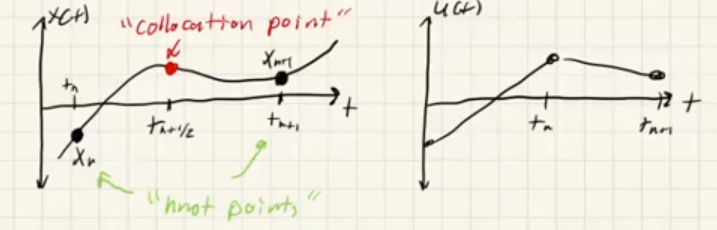
\includegraphics[width=0.4\linewidth]{L10_Images/F1.PNG}
    \caption{DIRCOL Spline Approximations}
    \label{fig:l10f1}
\end{figure}

\begin{itemize}
    \item So far we've used explicit RK methods to discretize dynamics:
    \begin{align}
        \dot x = f(x,u) \to x_{k+1} = f(x_k, u_k)
    \end{align}
    \item This makes sense if you're doing rollouts.
    \item However in a direct method where dynamics are enforced as equality constraints between knot points, this is not an advantage:
    \begin{align}
        c_k(x_k, u_k, x_{k+1}, u_{k+1}) = 0
    \end{align}
    \item Collocation methods represent trajectories with polynomial splines and enforce the dynamics on the spline derivatives.
    \item Classic DIRCOL algorithm uses cubic splines for state trajectories and piecewise linear interpolation for u(t).
    \item Very high-order polynomials are sometimes used (e.g. spacecraft trajectories), but not common.
    \item DIRCOL Spline Approximations:
    \begin{align}
        &x(t) = c_0 + c_1t + c_2 t^2 + c_3 t^3 \\
        &\dot x(t) = c_1 + 2 c_2 t + 3 c_3 t^2 \\
        &\begin{bmatrix}
            1 & 0 & 0 & 0 \\
            0 & 1 & 0 & 0 \\
            1 & h & h^2 & h^3 \\
            0 & 1 & 2h & 3h^2 \\
        \end{bmatrix}
        \begin{bmatrix}
            c_0 \\ c_1 \\ c_2 \\ c_3
        \end{bmatrix} = 
        \begin{bmatrix}
            x_k \\ \dot x_k \\ x_{k+1} \\ \dot x_{k+1}
        \end{bmatrix} \\
        &\begin{bmatrix}
            1 & 0 & 0 & 0 \\
            0 & 1 & 0 & 0 \\
            -3/h^2 & -2/h & 3/h^2 & -1/h \\
            2/h^3 & 1/h^2 & -2/h^3 & 1/h^2 \\
        \end{bmatrix}
        \begin{bmatrix}
            x_k \\ \dot x_k \\ x_{k+1} \\ \dot x_{k+1}
        \end{bmatrix} =
        \begin{bmatrix}
            c_0 \\ c_1 \\ c_2 \\ c_3
        \end{bmatrix}  
    \end{align}
    \item Evaluate at $t_{k+1/2}$
    \begin{align}
        x_{k+1/2} &= x(t_k + h/2) = \frac{1}{2}(x_k + x_{k+1}) + \frac{h}{8}(\dot x_k - \dot x_{k+1}) = \frac{1}{2}(x_k + x_{k+1}) + \frac{h}{8}(f(x_k, u_k) - f(x_{k+1}, u_{k+1})) \\
        \dot x_{k+1/2} &= \dot x(t_k + h/2) = -3/2h (x_k - x_{k+1}) - 1/4(\dot x_k + \dot x_{k+1}) = -3/2h(x_k - x_{k+1}) - 1/4(f(x_k, u_k) + f(x_{k+1}, u_{k+1})) \\
        u_{k+1/2} &= u(t_k + h/2) = \frac{1}{2}(u_k + u_{k+1})
    \end{align}
    \item We can now enforce dynamics constraints:
    \begin{align}
        c_i(x_k, u_k, x_{k+1}, u_{k+1}) = f(x_{k+1/2}, u_{k+1/2}) - (-3/2h(x_k - x_{k+1}) - 1/4(f(x_k, u_k) + f(x_{k+1}, u_{k+1})) = 0
    \end{align}
    \item Note that only $x_k, u_k$ are decision variables (not$x_{k+1/2}, u_{k+1/2}$)
    \item Called "Hermite-Simpson" integration.
    \item Achieve third prder accuracy like RK3.
    \item Requires fewer dynamics calls than explicit RK3!
    \item The Hermite-Simpson only 2 evals per time step!
    \item Since dynamics calls often dominate computational cost, this can be a 50\% savings.
\end{itemize}


\subsection{Recap: Deterministic Optimal Control Algorithm}
\begin{itemize}
    \item Linear/"Local" Control Problem.
    \begin{itemize}
        \item Without constraints: LQR
        \begin{itemize}
            \item Tracking: TVLQR
            \item Stabilization: TILQR
        \end{itemize}
        \item With constraints: MPC
        \begin{itemize}
            \item Linear Constraints: QP
            \item Conic Constraints: SOCP
        \end{itemize}
    \end{itemize}
    \item Nonlinear Trajectory Optimization/Planning
    \begin{itemize}
        \item DIRCOL:
        \begin{itemize}
            \item Only respects dynamics at convergence.
            \item Can supply infeasible guess.
            \item Can handle arbitrary constraints.
            \item Tracking controller must be designed separately.
            \item Typically not as fast.
            \item Difficult to implement large-scale SQP solver.
            \item Numerically robust.
        \end{itemize}
        \item DDP:
        \begin{itemize}
            \item Always dynamically feasible.
            \item Can only guess controls.
            \item Hard to handle constraints.
            \item TVLQR tracking controller is free.
            \item Very fast(local) convergence.
            \item Easy to implement on embedded systems.
            \item Has issue with ill-conditioning.
        \end{itemize}
        \item DDP is often a good choice for online/real-time applications where speed is critical and constraint tolerance is not critical.
        \item DIRCOL is often a good choice for offline trajectory design, especially over long horizons and/or with complex constraints.
    \end{itemize}
\end{itemize}






